% ============================================================
%  HOMEWORK REPORT TEMPLATE
%  Compile with: pdflatex homework_template.tex
% ============================================================
\documentclass[11pt, letterpaper]{article}

% ── Packages ────────────────────────────────────────────────
\usepackage[margin=1in]{geometry}
\usepackage{fancyhdr}
\usepackage{hyperref}
\usepackage{amsmath, amssymb}
\usepackage{enumitem}
\usepackage{booktabs}
\usepackage{xcolor}
\usepackage{setspace}
\usepackage{array}
\usepackage{graphicx}
\usepackage{subcaption}
\usepackage{multirow}
\usepackage{tabularx}
\usepackage{colortbl}
\usepackage{float}
\usepackage{placeins}
\usepackage{chngcntr}
\usepackage{lastpage}

% Load amsthm BEFORE parskip and titlesec to avoid patch conflict
\usepackage{amsthm}
\usepackage{parskip}

\usepackage{background}
\backgroundsetup{
  scale=8,
  angle=45,
  opacity=0.1,
  color=gray,
  contents={JSCHROEDER39}
}

\usepackage{titlesec}

\allowdisplaybreaks
\counterwithin*{equation}{subsection}

% ── Hyperlink Styling ────────────────────────────────────────
\hypersetup{
    colorlinks   = true,
    linkcolor    = black,
    urlcolor     = blue,
    citecolor    = black,
    pdftitle     = {Project Proposal},
}

% ── Header / Footer Setup ───────────────────────────────────
\pagestyle{fancy}
\fancyhf{}
\setlength{\headheight}{15pt}

\lhead{\textbf{\CourseName}}

\rhead{\AssignmentName}
\renewcommand{\headrulewidth}{1.2pt}
\cfoot{\thepage}
\renewcommand{\footrulewidth}{0pt}

% ── User-Defined Information ─────────────────────────────────
\newcommand{\StudentName}{Jacob Schroeder}
\newcommand{\TeamNumber}{42}
\newcommand{\CourseName}{ISYE6740: Computational Data Analysis}
\newcommand{\AssignmentName}{Project Proposal}
\newcommand{\AssignmentDue}{June 28, 2026}

% ── Section Formatting ──────────────────────────────────────
% Section: large bold, numbered "1.", rule beneath
\titleformat{\section}
    {\large\bfseries}
    {\thesection.}
    {0.5em}
    {}
    

% Subsection: normal size bold, numbered "1.1"
\titleformat{\subsection}
    {\normalsize\bfseries}
    {\thesubsection}
    {0.5em}
    {}

% ── Table of Contents Depth ─────────────────────────────────
\setcounter{tocdepth}{2}

% ============================================================
\begin{document}

% ── COVER PAGE ──────────────────────────────────────────────
\thispagestyle{empty}
\begin{center}
    \vspace*{1.5cm}

    {\Huge \textbf{\AssignmentName}}\\[0.6cm]
    {\large \CourseName}\\[0.4cm]
    \rule{0.6\textwidth}{0.8pt}\\[0.8cm]

    \begin{tabular}{>{\bfseries}r l}
        Name:        & \StudentName   \\[4pt]
        Team Number:  & \TeamNumber     \\[4pt]
        Due Date:    & \AssignmentDue \\[4pt]
    \end{tabular}

    \vspace{1.2cm}
    \rule{0.6\textwidth}{0.8pt}
\end{center}

% ── TABLE OF CONTENTS ───────────────────────────────────────
\newpage
\thispagestyle{fancy}
\tableofcontents

% ============================================================
%  PROBLEMS BEGIN HERE
% ============================================================

\newpage
\section{Introduction}

LEGO has a fascinating history. Originating in Denmark in 1932, it began as a small wooden toy manufacturer. Since then it has grown into one of the most iconic toys ever produced. The LEGO brick as we know it today was introduced in 1958, and since then the brand has released thousands of distinct sets spanning dozens of licensed and original themes. Everything from the earliest Town and Castle series released in the 1970s, to the endlessly popular Star Wars licensed sets released beginning in the late 1990s, to the adult-targeted Icons and Architecture lines released for those of us who haven't fully grown up yet each set comes with hundreds of individual parts, colors, minifigures and other characteristics that make it both distinct and part of a greater collection.

Over the years, LEGO sets have evolved in piece count, colors, set complexity, and other key changes that make LEGO what they are. Things like the first lego sets with instructions being introduced in 1964, LEGO Technic introducing an entirely new style of piece getting added in 1977, the first Start Wars licensed set released in 1999, and robotics getting added with LEGO Mindstorms in 2006 have all been critical additions which have shaped the brand and the composition of those sets. This project will examine that composition and how it has changed over the years.

\section{Problem Statement}

\textit{Can unsupervised machine learning detech meaningul structural shifts in LEGO set design over time, and do those detected shifts correspond to known historical events in the company's history?}

This is the question that this project will attempt to answer using temporal clustering \cite{chi2007evolutionary} and distributional drift detection \cite{gama2014survey}. Over the past several decades, LEGO has expanded from a company focusing primarily on traditional building sets to a global entertainment brand ecompassing licensed franchises, collector-focused products, and highly specialized themes. These changes are incredibly well documented from a business perspective, but it can be very uncelar how LEGO's product designs have evolved over time when viewed solely through the characteristics of the sets. 

The objective of this project will be to analyze the evolution of LEGO products from the 1950s through the present day using unsupervisded machine learning techniques. Specifically, LEGO sets will be grouped into clusters based on structural and design-related features and the analysis will examine how these clusters change over time. When looking at the shifts in the composition of clusters across different years, the expectation is that certain substaintial changes will appear aligning with major changes to LEGO's product portfolio. 

\section{Proposed Methodology}

\subsection{Data Source and Preprocessing}

Data will be sourced from the Rebrickable database \cite{rebrickable2024}, which provides both API and CSV exports for all lego set related data. For this project, I will use the CSV export of a large relational database including the following tables: \texttt{sets}, \texttt{themes}, \texttt{parts}, \texttt{part\_categories}, \texttt{colors}, \texttt{inventories}, \texttt{inventory\_parts}, \texttt{inventory\_minifigs}, and \texttt{minifigs}. The complete entity relationship diagram including all attributes can be found in the appendix. These will be loaded into a local SQLite database via Python's \texttt{sqlite3} module and queried using \texttt{pandas} for downstream processing. 

Sets with a very small number of parts will be excluded as non-standard releases (e.g., promotional packs, individual minifigures, individual parts sold as set). Additionally, years with a small number of sets released in the catalog will be grouped using rolling windows to ensure a large enough cohort size for stable clustering.

\subsection{Feature Engineering}

Each set $s_i$, will be represented by a $d$-dimensional feature vector capturing structural properties at multiple levels of abstraction: 

\begin{itemize}
    \item \textbf{Scale features:} total part count, unique part count, minifigure count, spare part ratio
    \item \textbf{Diversity features:} Shannon entropy of part categories $H_\text{cat}$, Shannon entropy of colors $H_\text{col}$, number of distinct colors, number of distinct part categories
    \item \textbf{Composition features:} proportion of Technic parts, proportion of decorative/printed parts, proportion of transparent parts (via \texttt{colors.is\_trans}), rare part ratio (parts appearing in fewer than 20 sets total)
    \item \textbf{Minifigure features:} minifigure-to-part ratio, binary indicator for presence of minifigures
\end{itemize}

All features will be normalized prior to clustering and highly correlated features will be removed to reduce redundancy.

\subsection{Dimensional Reduction}

Each set $s_i$ will be reduced from its $d$-dimensional feature space into a feature space of 2-3 dimensions for visualization purposes. The method of this reduction has not yet been determined. Currently, I am exploring using either UMAP \cite{mcinnes2018umap} or PCA. Currently, I am leaning towards UMAP as it preserves local neighborhood structure better. This will be advantageous when identifying clusters when performing visualizations. The reduced representation will be used for visualization only while clustering will be performed on the full feature space.

\subsection{Temporal Clustering}

For each time cohort $\mathcal{C}_t$, $k$-means clustering will be applied with $k$ selected via the elbow method and silhouette score analysis on the first available cohort. These will remain fixed across the years to enable centroid comparison. 

A follow up comparison to the which may be interesting to conduct should time an computing power allow will be to compare the optimal number of clusters across years. This will be a secondary research question where we see how the number of clusters grows compared to the number of collections. 

\subsection{Drift Detection}

The dissimilarity between consectuive clustering solutions will be be measured using two metrics:

\begin{enumerate}
    \item \textbf{Adjusted Rand Index (ARI):} For sets present in both cohorts $\mathcal{C}_t$ and $\mathcal{C}_{t+1}$ (overlapping years), ARI will measure the agreement between the two clustering assignments. A sharp drop in ARI signals structural reorganization \cite{mishra2025cluster}.
    \item \textbf{Centroid displacement:} The average Euclidean distance between matched centroid pairs $\|\mu_j^{(t+1)} - \mu_j^{(t)}\|_2$, averaged over all $k$ clusters, captures smooth directional drift even when set membership does not overlap between cohorts.
\end{enumerate}

\subsection{Reproducibility}

All code will be written in Python and made available alongside the SQLite database construction scripts. Random seeds will be fixed at 42 (the meaning of life, the universe, and everything) to ensure reproducible random cluster initializations. 

\section{Evaluation Strategies}

\subsection{Internal Clustering Validity}

For each annual clustering solution $\mathcal{K}_t$, internal quality will be assessed using:
\begin{itemize}
    \item \textbf{Silhouette score:} Measures how similar each point is to its own cluster relative to other clusters; scores near $1$ indicate well defined clusters \cite{rousseeuw1987silhouettes}.
    \item \textbf{Davies-Bouldin Index:} Penalizes clusters that are large and close together; lower values indicate better separation.
    \item \textbf{Elbow method on inertia:} Confirms that the chosen $k$ is appropriate and stable across years.
\end{itemize}

Consistency of these metrics across years will itself be informative: a sudden degradation in silhouette score in a given year suggests the data no longer conforms to the assumed cluster geometry, which is an independent signal of drift.

\subsection{External Validation Against Theme Labels}

Although theme labels are not used as features, they can be used for external validations. After fitting each annual clustering, I will compute:
\begin{itemize}
    \item \textbf{Normalized Mutual Information (NMI)} between cluster assignments and official theme labels
    \item \textbf{Homogeneity and completeness scores} to assess whether clusters align with the theme.
\end{itemize}

\section{Conclusion}

LEGO has long been a passion of mine from a very young age. While my appreciationn for the brand and the product began as a child, it has remained a hobby well into adulthood. My growth reflects LEGOs growth. When I was younger, I thought that LEGO Star Wars was the greatest thing on earth. While I still love those sets, my passions have shifted towards the large-scale car models like the Formula 1 cars, Porsche 911, Land Rover Defender, as well as the new LEGO Lord of the Rings collection.

This project gives me a great opportunity to combine a personal passion for LEGO with the machine learning techniques studied in this course. By applying clustering and drift detection methods to decades of LEGO set data, I hope to uncover patterns in the evolution of the brand and show how the composition of the product design which has made this iconic brand so successful reveals shifts not obvious to the human eye.



\newpage

\section{Appendix}

\subsection{Rebrickable Entity Relationship Diagram}

\begin{figure}[h]
  \centering
  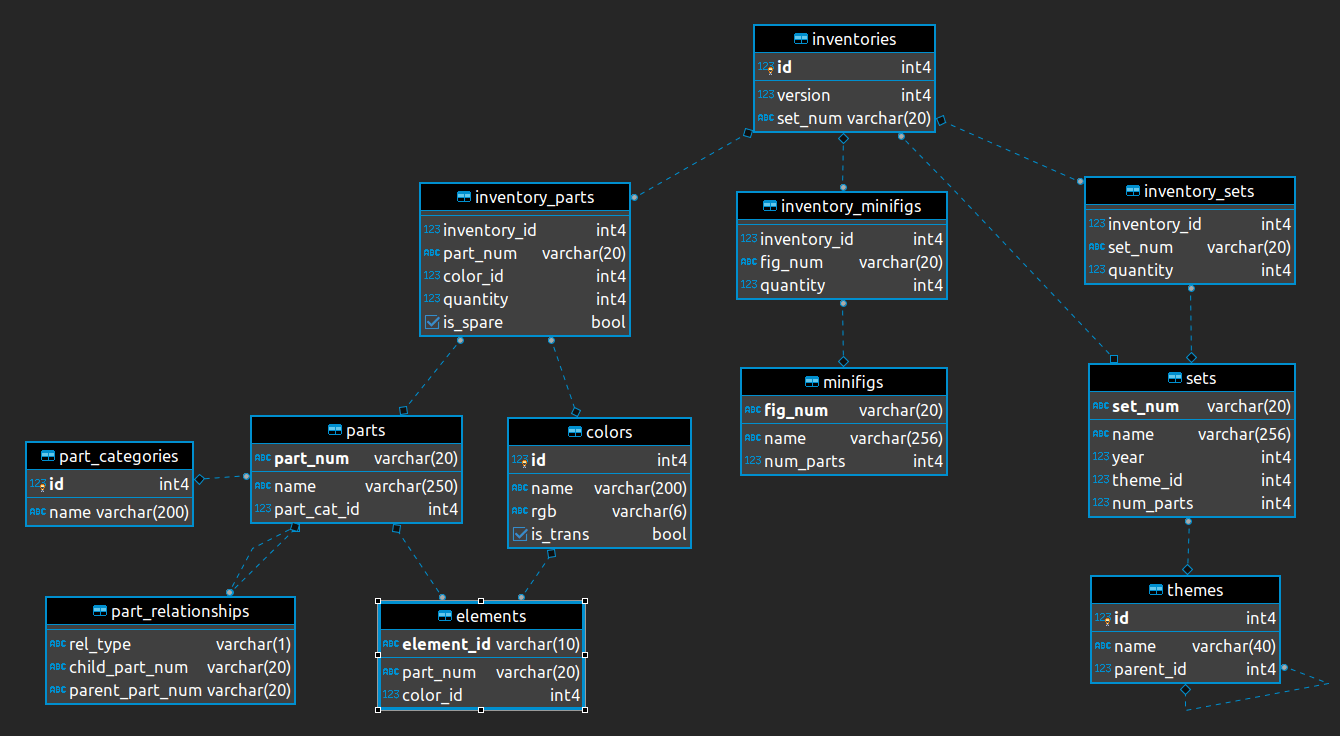
\includegraphics[width=1\textwidth]{images/ERD.png}
    \caption{Database schema for the Rebrickable \cite{rebrickable2024} LEGO dataset. The relational structure links LEGO sets to inventories, parts, colors, themes, and minifigures, providing the foundation for feature engineering and longitudinal analysis of changes in LEGO product design over time}
\end{figure}

\newpage

\addcontentsline{toc}{section}{References}
\bibliographystyle{plain}
\bibliography{references}

\begin{thebibliography}{9}

\bibitem{chi2007evolutionary}
Chi, Y., Song, X., Zhou, D., Hino, K., \& Tseng, B. L. (2007).
\newblock Evolutionary spectral clustering by incorporating temporal smoothness.
\newblock In \textit{Proceedings of the 13th ACM SIGKDD International Conference on Knowledge Discovery and Data Mining} (pp. 153--162).
\newblock \url{https://doi.org/10.1145/1281192.1281212}

\bibitem{gama2014survey}
Gama, J., Žliobaitė, I., Bifet, A., Pechenizkiy, M., \& Bouchachia, A. (2014).
\newblock A survey on concept drift adaptation.
\newblock \textit{ACM Computing Surveys}, 46(4), 1--37.
\newblock \url{https://doi.org/10.1145/2523813}

\bibitem{mcinnes2018umap}
McInnes, L., Healy, J., \& Melville, J. (2018).
\newblock UMAP: Uniform manifold approximation and projection for dimension reduction.
\newblock \textit{arXiv preprint arXiv:1802.03426}.
\newblock \url{https://arxiv.org/abs/1802.03426}

\bibitem{mishra2025cluster}
Mishra, A., \& Stamp, M. (2025).
\newblock Cluster analysis and concept drift detection in malware.
\newblock \textit{arXiv preprint arXiv:2502.14135}.
\newblock \url{https://arxiv.org/abs/2502.14135}

\bibitem{rebrickable2024}
Rebrickable. (2024).
\newblock LEGO sets database downloads.
\newblock \url{https://rebrickable.com/downloads/}

\bibitem{rousseeuw1987silhouettes}
Rousseeuw, P. J. (1987).
\newblock Silhouettes: A graphical aid to the interpretation and validation of cluster analysis.
\newblock \textit{Journal of Computational and Applied Mathematics}, 20, 53--65.
\newblock \url{https://doi.org/10.1016/0377-0427(87)90125-7}

\end{thebibliography}

\end{document}